\documentclass[conference]{IEEEtran}
\IEEEoverridecommandlockouts

\usepackage{cite}
\usepackage{amsmath,amssymb,amsfonts}
\usepackage{graphicx}
\usepackage{textcomp}
\usepackage{xcolor}
\usepackage{booktabs}
\usepackage{url}
\usepackage{array}
\usepackage{float}

\def\BibTeX{{\rm B\kern-.05em{\sc i\kern-.025em b}\kern-.08em
    T\kern-.1667em\lower.7ex\hbox{E}\kern-.125emX}}

\begin{document}

\title{Measuring HPC Efficiency with PEAK: How Well Do Your Tools Use Supercomputer Resources?}

\author{
\IEEEauthorblockN{Caleb Wiyninger}
\IEEEauthorblockA{
\textit{Dept. of Computer Science, Oklahoma City University} \\
\textit{REU Intern, Texas Advanced Computing Center} \\
Oklahoma City, OK / Austin, TX, USA \\
cwiyninger@my.okcu.edu}
\and
\IEEEauthorblockN{Chun-Yaung Lu (Albert)}
\IEEEauthorblockA{
\textit{Texas Advanced Computing Center} \\
\textit{The University of Texas at Austin} \\
Austin, TX, USA \\
alu@tacc.utexas.edu}
\and
\IEEEauthorblockN{Yinzhi Wang (Ian)}
\IEEEauthorblockA{
\textit{Texas Advanced Computing Center} \\
\textit{The University of Texas at Austin} \\
Austin, TX, USA}
}

\maketitle

\begin{abstract}
High Performance Computing (HPC) systems and the science, math, and machine learning programming libraries optimized for those systems are essential for accelerating large-scale scientific research. Maximizing the performance of these libraries is critical for enabling faster scientific discovery. Using the Performance Evaluation and Analysis Kit (PEAK) and usage data gathered from the Texas Advanced Computing Center (TACC), this project profiles several widely utilized science and math toolkits, including ABINIT, DFTB+, and GROMACS, to evaluate how efficiently they utilize standard numerical libraries such as BLAS, LAPACK, and FFTW across the diverse operational contexts common to HPC environments. By employing a cost-adaptive profiling strategy that balances accuracy and overhead trade-offs via dynamic library preloading, the expected outcome is to capture critical performance data points and library invocation frequencies that traditional profilers miss. At the conclusion of testing, the expectation is to identify specific computational bottlenecks and ideal operational conditions to deliver concrete optimization recommendations. This analysis will provide a definitive framework for the future design of high-performance computing infrastructure and tools prioritizing maximum runtime efficiency, ultimately reducing core-hour expenditure and accelerating computational workflows for the broader scientific community.
\end{abstract}

\begin{IEEEkeywords}
high performance computing, profiling, PEAK, BLAS, LAPACK, FFTW, benchmarking, scientific computing
\end{IEEEkeywords}

\section{Introduction}

\subsection{Broad Context}
High Performance Computing (HPC) systems are critical tools for accelerating large scale scientific research. These systems are built from many interconnected computers referred to as nodes. Due to this unique architecture, programs must be designed specifically to take advantage of these resources.

\subsection{The Problem}
In order to optimize for these environments, many things must be known about a program: what other software it relies on, where a majority of computation time is spent, how different amounts and types of resources affects performance, and the impact of different variables on performance.

\subsection{The Solution}
Using usage data from the Texas Advanced Computing Center (TACC), the Performance Evaluation and Analysis Kit (PEAK), and the Stampede3 supercomputer, we can analyze some of the most used scientific software to determine how well they utilize HPC resources and get a deeper insight into where the programs are spending their time.

\subsection{Roadmap}
This paper will provide an overview of how modern HPC systems work, what problems they introduce for optimization, where these programs spend their time, what libraries these programs rely on, and how well these programs take advantage of HPC resources. Section II will provide a brief overview of HPC systems and the challenges they introduce as well as an introduction to the PEAK tool. Section III will provide an overview of the approach of how we select, build, test, scale, and analyze the programs. Section IV will present our results. Section V will provide a discussion of our results and what they mean for the programs we analyzed. Section VI will highlight some of our limitations and explain how we plan to address them among other future work. Section VII will provide a conclusion and summary of our findings.

\section{Background}

\subsection{HPC Systems}
Most modern HPC systems are built upon a cluster computing architecture, this means that they are made up of many interconnected computers referred to as nodes. These nodes vary in hardware, purpose, and performance but all are meant to work together to solve large scale problems. In order to run a program on an HPC system, a scheduler is used to allocate resources and manage the execution of the program. A user must submit a job script to the scheduler that specifies the resources needed and the program to be run and the scheduler will then allocate the resources and run the program on the allocated nodes.

\subsection{Prior Work}

\subsubsection{PEAK}
PEAK is a tool designed for HPC systems that allows the user to analyze a target program for function calls, where compute time is spent, and how the targeted program utilizes popular mathematical libraries such as BLAS (Basic Linear Algebra Subprograms), LAPACK (Linear Algebra PACKage), and FFTW (Fastest Fourier Transform in the West). PEAK uses the Frida-Gum toolkit to inject monitoring code into running binaries and dynamically attaches and detaches to stay below a specified level of overhead. This allows for PEAK to provide more accurate results while still keeping overhead low. PEAK is configured via environmental variables and invoked via \texttt{LD\_PRELOAD}. Due to PEAK being in active development, this study also provides useful feedback directly to the PEAK team on usage experience, documentation, and bugs.

\subsubsection{BenchPRO}
Benchmark Performance and Reproducibility Orchestrator (BenchPRO) is a tool designed to run reproducible benchmarks. The goals of BenchPRO and this study overlap, but we opted for a from-scratch approach in order to have more control over individual configurations and to better understand the underlying processes and techniques for performance benchmarking.

\section{Approach}
A list of the 100 program names, sorted by core hour used, gathered from the Frontera supercomputer was trimmed of unactionable names such as duplicates, language interpreters, or generic names into a list of actionable names. We added more programs to this list based on our own knowledge of popular scientific software. Cursory research was done on each program in order to determine domain, purpose, and if TACC had a prebuilt version of the program available. LLMs were used to assist in this research. There are currently 67 programs and counting in this list.

\subsection{Environment}
All programs were run on the Stampede3 supercomputer at TACC using nodes equipped with 48 core Intel Xeon Platinum 8160 (``Skylake'') processors and 192 GB of RAM.

\subsection{Build Scripts and Modules}
Some programs were available as prebuilt modules maintained by TACC, while others required building from source. In order to keep binaries reproducible and identical, we opted for TACC's modules when available and created build scripts when they were not.

\subsection{Test Cases and Input}
For each program, we chose or created a test case that would run in a reasonable amount of time and represent a typical use case for the program. When available, we sourced our test cases from a program's pre-bundled test cases or third party test cases. When those sources were unavailable, we created our own test cases. Due to the in-depth knowledge required to create or modify a test case for a program, LLMs were used to assist in creating and modifying test cases.

\subsection{Scaling}
Programs were run at a series of different scales, starting with a single node and scaling up to 16 nodes. Single node scaling was done at 1, 24, and 48 cores. Multi-node scaling was done at 2, 8, and 16 nodes with 48 cores per node.

\subsection{Automation Scripts}
In order to speed up research, a reusable bash script was created to automatically generate the needed job scripts for each program, scale, and test case. The script read from a configuration file that specified the program, scale, and test cases to be run. Another job was created to run the target program with PEAK attached and configured to profile for BLAS, LAPACK, and FFTW function calls. Another script was created to consolidate similar jobs into job arrays to reduce the number of jobs submitted to the scheduler, allowing for more jobs to be submitted at once. All jobs were organized into directories based on program name, scale, and test case for easy access and analysis. All jobs included timing logging and automatically appended data to a main summary file.

\subsection{Visualization}
In order to understand our results, we created a python script to parse the summary files and generate visualizations of the data.

\section{Results}

\subsection{ABINIT}
\textbf{Description:} Simulates how electrons and atoms behave in materials, using quantum mechanics to predict a material's structure, energy, and properties.\\
\textbf{Test Case:} Simulating a silicon crystal.

\begin{table}[H]
\centering
\caption{ABINIT Job Summary}
\label{tab:abinit-summary}
\scriptsize
\begin{tabular}{c c c c}
\toprule
Nodes & Tasks & PEAK & Elapsed (s) \\
\midrule
1  & 1   & No  & 119 \\
1  & 24  & No  & 10  \\
1  & 48  & No  & 8   \\
2  & 96  & No  & 6   \\
8  & 384 & No  & 6   \\
16 & 768 & No  & 9   \\
1  & 1   & Yes & 126 \\
\bottomrule
\end{tabular}
\end{table}

\begin{table}[H]
\centering
\caption{ABINIT PEAK Results}
\label{tab:abinit-peak}
\scriptsize
\begin{tabular}{l r r r r}
\toprule
Function & Calls & \shortstack{Total\\Time (s)} & \shortstack{Avg. Time\\/Call (ms)} & \shortstack{PEAK\\Overhead (s)} \\
\midrule
\texttt{zgemm\_}  & 207,990 & 4.7613 & 0.0229 & 0.4258 \\
\texttt{ddot\_}   & 216,544 & 0.6383 & 0.0029 & 0.4433 \\
\texttt{zcopy\_}  & 131,022 & 0.6081 & 0.0046 & 0.2682 \\
\texttt{dznrm2\_} & 116,280 & 0.5958 & 0.0051 & 0.2380 \\
\texttt{zdotc\_}  & 51,588  & 0.1846 & 0.0036 & 0.1056 \\
\bottomrule
\end{tabular}
\end{table}

\begin{figure}[H]
\centering

\includegraphics[width=\columnwidth]{abinit_fullPEAK-scaling-07102026-152428_dashboard.png}
\caption{ABINIT scaling and PEAK results.}
\label{fig:abinit}
\end{figure}

\subsection{Quantum Espresso}
\textbf{Description:} Quantum-mechanical materials simulation package, solving the same kind of problem as ABINIT with a different underlying computational method.\\
\textbf{Test Case:} Simulating a silicon crystal.

\begin{table}[H]
\centering
\caption{Quantum Espresso Job Summary}
\label{tab:qe-summary}
\scriptsize
\begin{tabular}{c c c c}
\toprule
Nodes & Tasks & PEAK & Elapsed (s) \\
\midrule
1  & 1   & No  & 636 \\
1  & 24  & No  & 63  \\
1  & 48  & No  & 34  \\
2  & 96  & No  & 28  \\
8  & 384 & No  & 20  \\
16 & 768 & No  & 27  \\
1  & 1   & Yes & 638 \\
\bottomrule
\end{tabular}
\end{table}

\begin{table}[H]
\centering
\caption{Quantum Espresso PEAK Results}
\label{tab:qe-peak}
\scriptsize
\begin{tabular}{l r r r r}
\toprule
Function & Calls & \shortstack{Total\\Time (s)} & \shortstack{Avg. Time\\/Call (ms)} & \shortstack{PEAK\\Overhead (s)} \\
\midrule
\texttt{zgemm\_}  & 144,849 & 166.6082 & 1.1502 & 0.2227 \\
\texttt{zhegvx\_} & 5,561   & 8.3896   & 1.5087 & 0.0085 \\
\texttt{zgemv\_}  & 1,184   & 3.7863   & 3.1979 & 0.0018 \\
\texttt{ddot\_}   & 57,984  & 0.3923   & 0.0068 & 0.0891 \\
\texttt{dcopy\_}  & 1,926   & 0.3207   & 0.1665 & 0.0030 \\
\bottomrule
\end{tabular}
\end{table}

\begin{figure}[H]
\centering
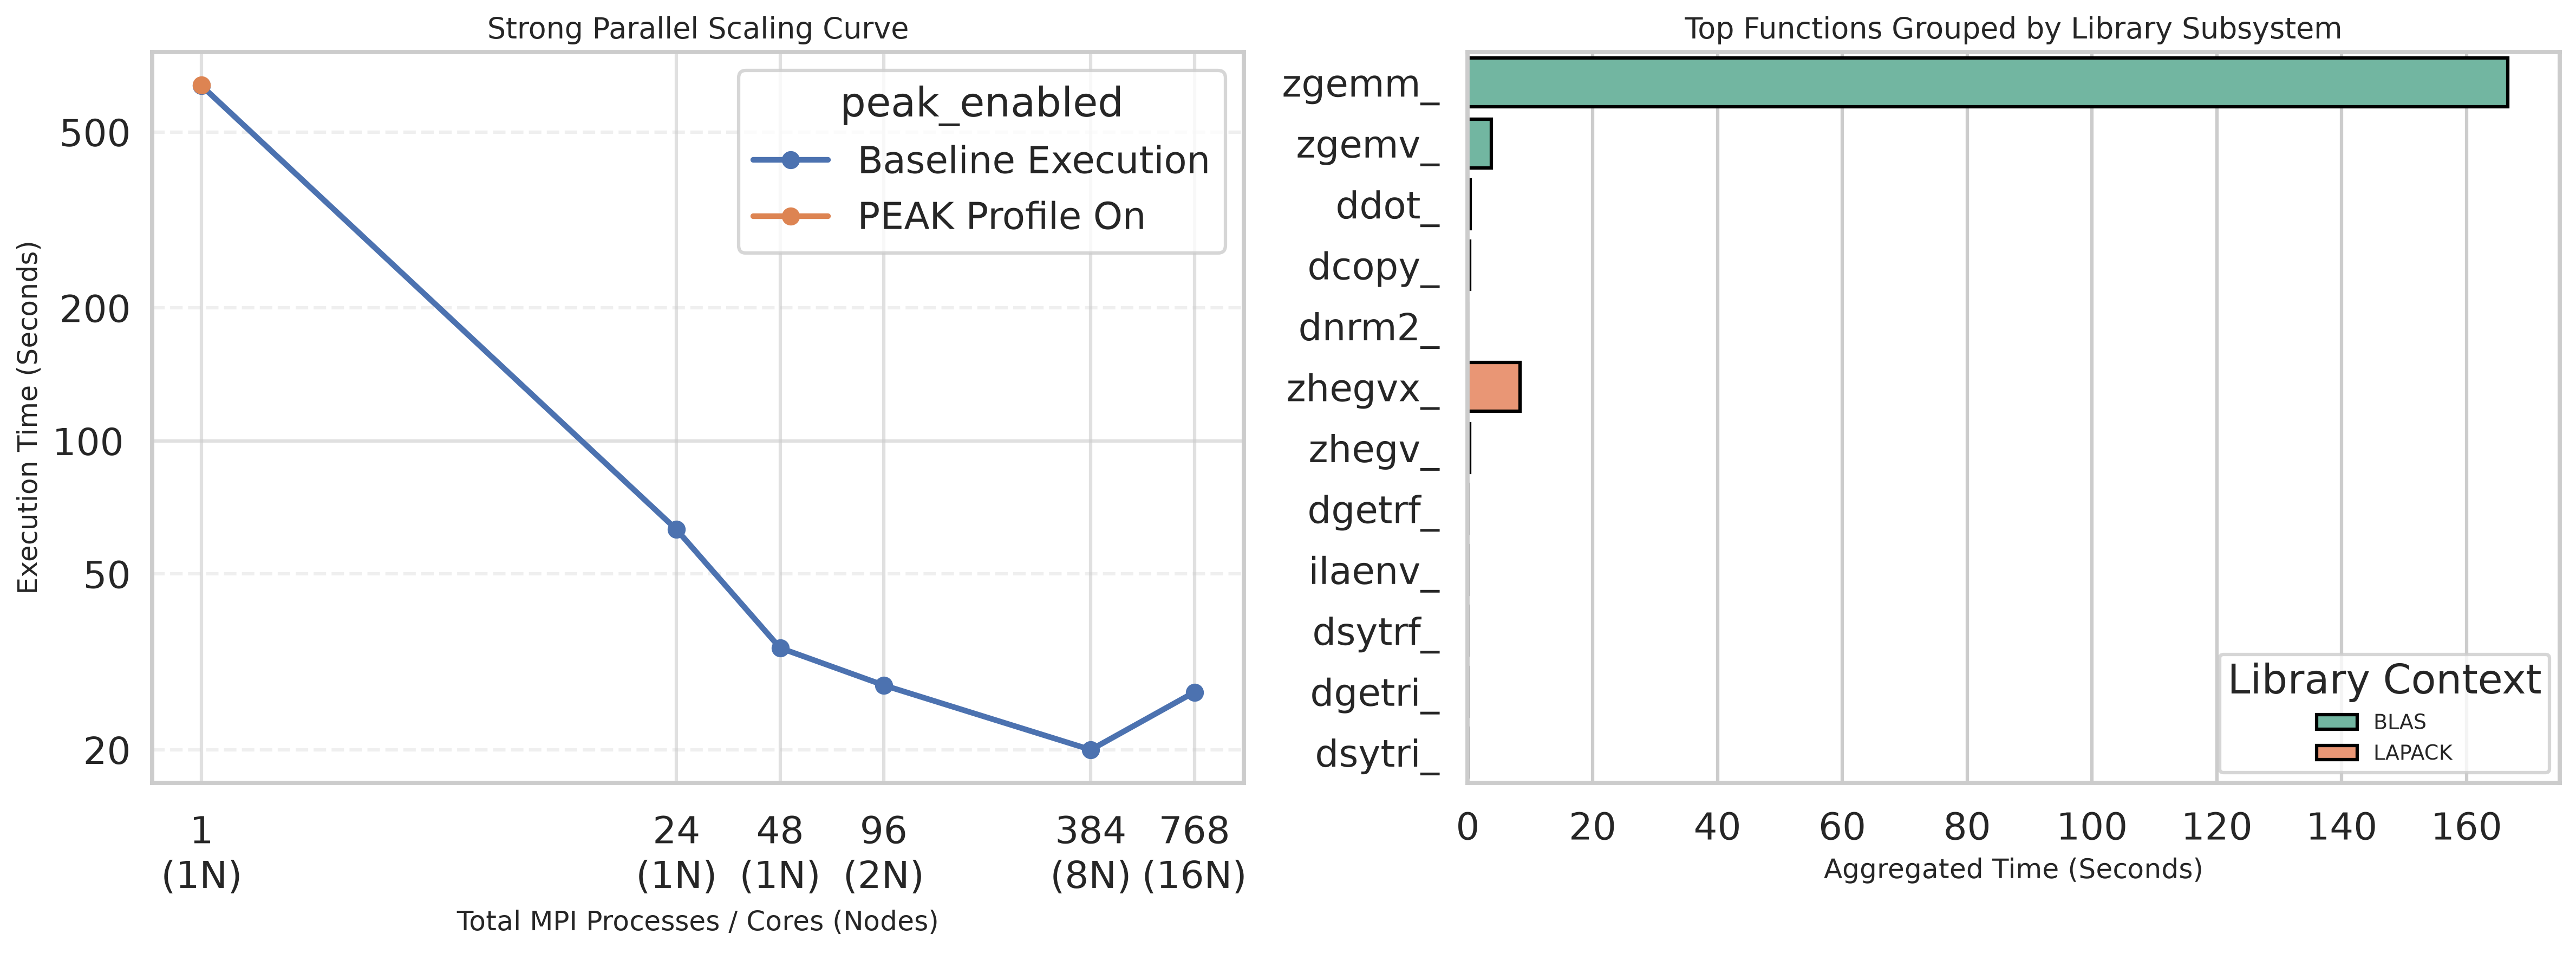
\includegraphics[width=\columnwidth]{qe_fftw_test-scaling-07142026-092819_dashboard.png}
\caption{Quantum Espresso scaling and PEAK results.}
\label{fig:qe}
\end{figure}

\subsection{DFTB+}
\textbf{Description:} A faster, approximate alternative to full quantum-mechanical simulation, trading some accuracy for greatly reduced compute time.\\
\textbf{Test Case:} Simulating a carbon molecule.

\begin{table}[H]
\centering
\caption{DFTB+ Job Summary}
\label{tab:dftb-summary}
\scriptsize
\begin{tabular}{c c c c}
\toprule
Nodes & Tasks & PEAK & Elapsed (s) \\
\midrule
1  & 1   & No  & 120 \\
1  & 24  & No  & 144 \\
1  & 48  & No  & 220 \\
1  & 1   & Yes & 121 \\
2  & 96  & No  & 2\textsuperscript{*} \\
8  & 384 & No  & 3\textsuperscript{*} \\
16 & 768 & No  & 3\textsuperscript{*} \\
\bottomrule
\end{tabular}
\\[2pt]
\raggedright\scriptsize\textsuperscript{*}Job exited with a non-zero exit code (1); reported elapsed time reflects time-to-crash, not completion.
\end{table}

\begin{table}[H]
\centering
\caption{DFTB+ PEAK Results}
\label{tab:dftb-peak}
\scriptsize
\begin{tabular}{l r r r r}
\toprule
Function & Calls & \shortstack{Total\\Time (s)} & \shortstack{Avg. Time\\/Call (s)} & \shortstack{PEAK\\Overhead (s)} \\
\midrule
\texttt{dsyev\_}  & 4      & 94.1030 & 23.5258 & 0.0000 \\
\texttt{dgemm\_}  & 442    & 10.5098 & 0.0238  & 0.0007 \\
\texttt{dsymm\_}  & 4      & 10.0370 & 2.5092  & 0.0000 \\
\texttt{dlarrv\_} & 4      & 0.1037  & 0.0259  & 0.0000 \\
\texttt{dcopy\_}  & 34,760 & 0.0280  & 0.0008  & 0.0541 \\
\bottomrule
\end{tabular}
\end{table}

\begin{figure}[H]
\centering
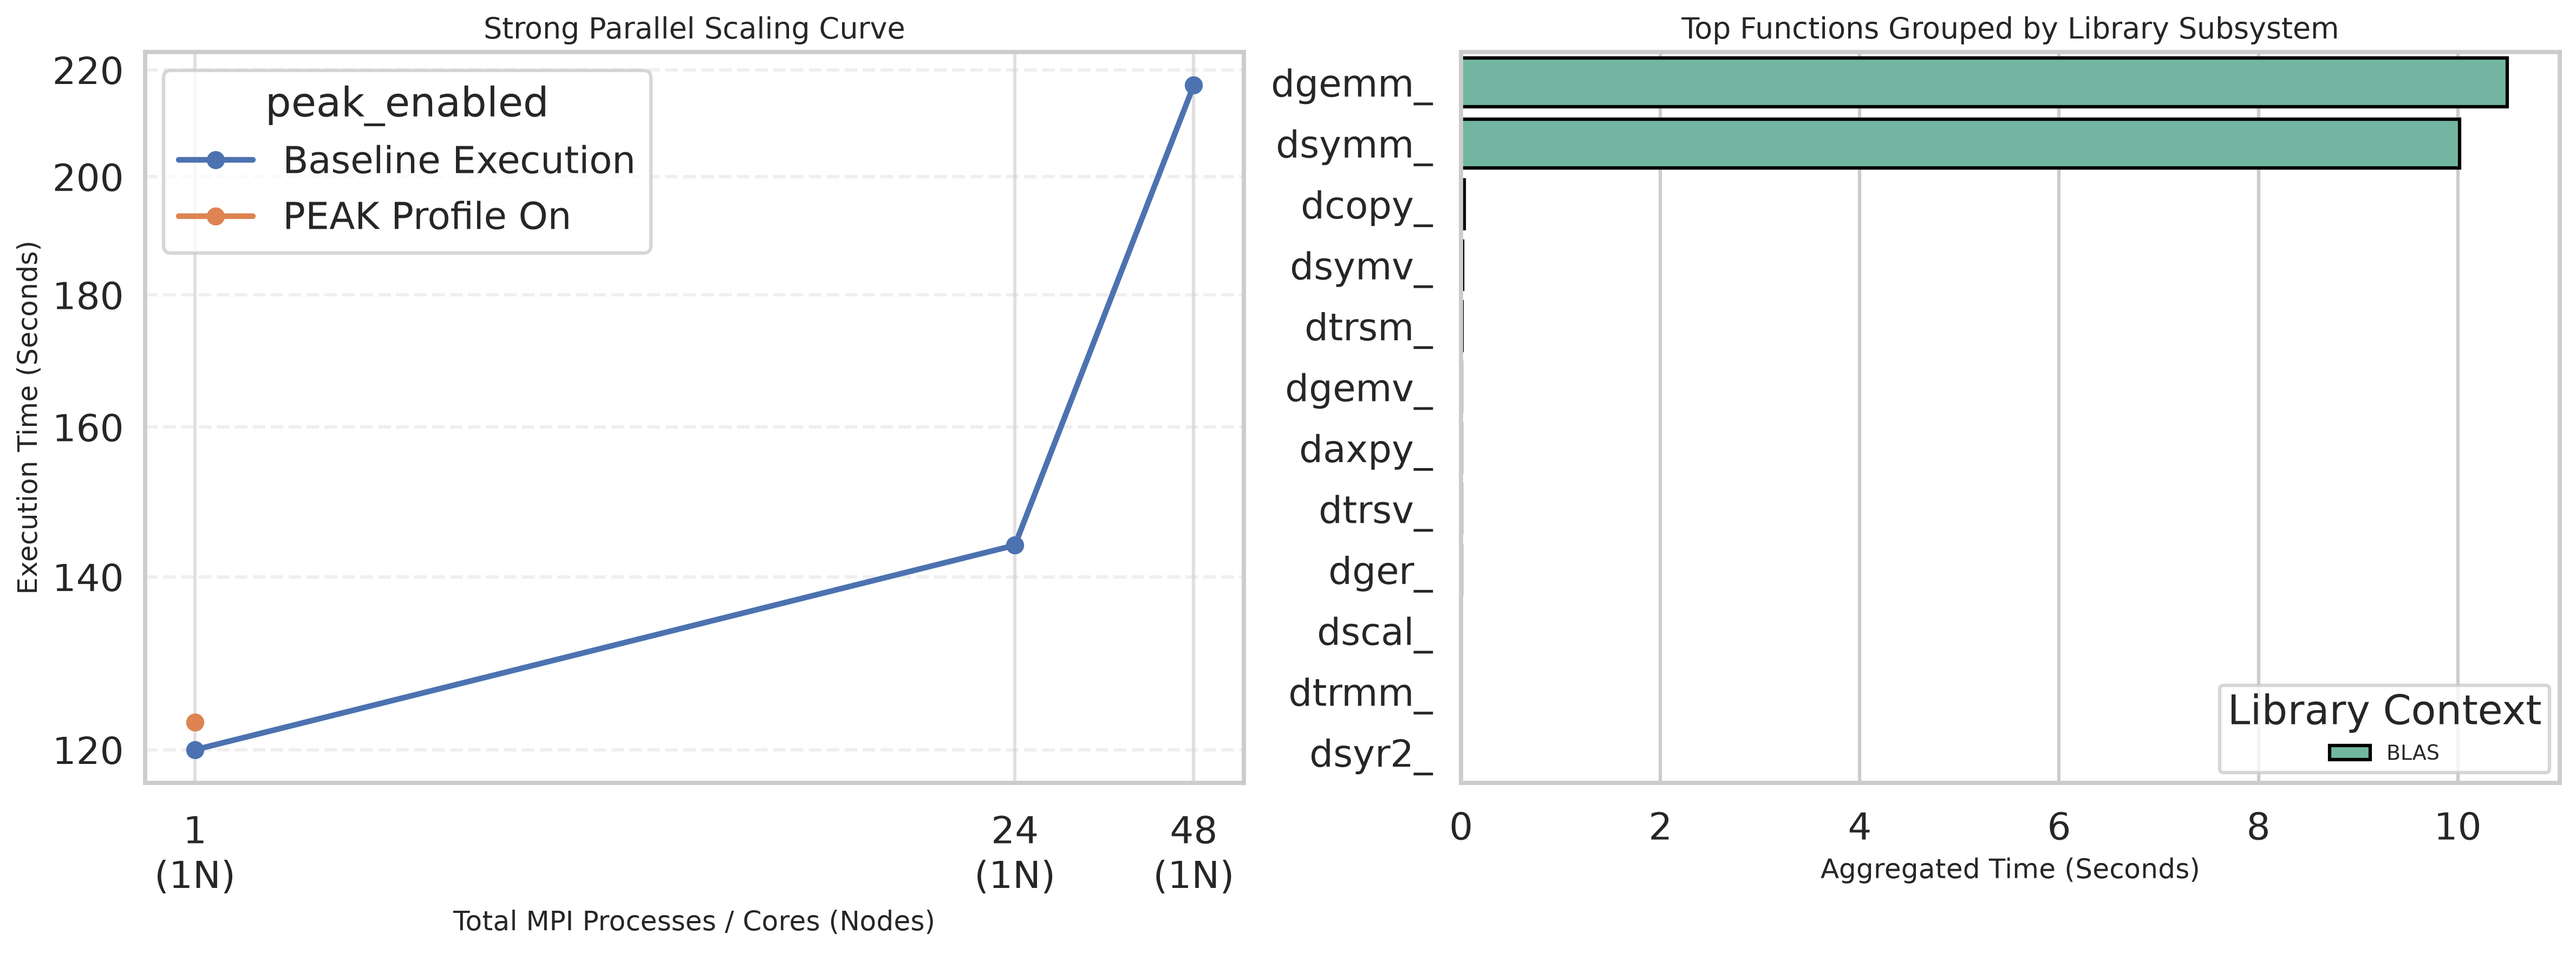
\includegraphics[width=\columnwidth]{dftb_2_peak_target_config-scaling-07142026-144018_dashboard.png}
\caption{DFTB+ scaling and PEAK results.}
\label{fig:dftb}
\end{figure}

\subsection{GROMACS}
\textbf{Description:} Simulates the motion and interactions of biomolecules like proteins and lipids, widely used to study biological and chemical processes.\\
\textbf{Test Case:} Simulating protein in a membrane.

\begin{table}[H]
\centering
\caption{GROMACS Job Summary}
\label{tab:gromacs-summary}
\scriptsize
\begin{tabular}{c c c c}
\toprule
Nodes & Tasks & PEAK & Elapsed (s) \\
\midrule
1  & 24  & No  & 213 \\
1  & 48  & No  & 125 \\
1  & 48  & Yes & 126 \\
2  & 96  & No  & 75  \\
8  & 384 & No  & 37  \\
16 & 768 & No  & 36  \\
\bottomrule
\end{tabular}
\end{table}

\textit{PEAK Results:} This build of GROMACS did not yield any PEAK hits.

\begin{figure}[H]
\centering

\includegraphics[width=\columnwidth]{gromacs_2-scaling-07102026-221528_dashboard.png}
\caption{GROMACS scaling results.}
\label{fig:gromacs}
\end{figure}

\subsection{LAMMPS}
\textbf{Description:} Simulates how large numbers of atoms and molecules move and interact over time (molecular dynamics), commonly used to study materials at the atomic scale.\\
\textbf{Test Case:} Simulating protein in a membrane.

\begin{table}[H]
\centering
\caption{LAMMPS Job Summary}
\label{tab:lammps-summary}
\scriptsize
\begin{tabular}{c c c c}
\toprule
Nodes & Tasks & PEAK & Elapsed (s) \\
\midrule
1  & 1   & No  & 32 \\
1  & 24  & No  & 4  \\
1  & 48  & No  & 4  \\
2  & 96  & No  & 4  \\
8  & 384 & No  & 4  \\
16 & 768 & No  & 8\textsuperscript{*} \\
1  & 1   & Yes & 32 \\
\bottomrule
\end{tabular}
\\[2pt]
\raggedright\scriptsize\textsuperscript{*}Job exited with a non-zero exit code (255).
\end{table}

\textit{PEAK Results:} This build of LAMMPS did not yield any PEAK hits.

\begin{figure}[H]
\centering

\includegraphics[width=\columnwidth]{lammps_5-scaling-07132026-225745_dashboard.png}
\caption{LAMMPS scaling results.}
\label{fig:lammps}
\end{figure}

\section{Discussion}

\subsection{ABINIT}
ABINIT scaled effectively from 1 to 384 tasks (119s to 6s), but got slightly worse at 768 tasks (9s). This is most likely due to inter-node communication overhead. This is a common problem in HPC systems, where the time spent communicating between nodes can outweigh the benefits of adding more resources. This run represents what we would expect from most programs, where more resources leads to better performance, but only up to a certain point. ABINIT relies heavily on BLAS and somewhat on LAPACK. A majority of compute is spent on the \texttt{zgemm\_} function, which is a BLAS function for matrix multiplication.

\subsection{Quantum Espresso}
Quantum Espresso scales well up to 384 tasks (636s to 20s), then degrades at 768 tasks (27s). This is a similar story to ABINIT, where the program scales well up to a certain point, but then suffers from inter-node communication overhead. Quantum Espresso's PEAK results resemble ABINIT's, with a majority of compute time spent on the \texttt{zgemm\_} function, which is a BLAS function for matrix multiplication.

\subsection{DFTB+}
The most interesting result from our study was DFTB+, which performed worse with more resources and outright crashed when multiple nodes were introduced. This is a clear example of a program that does not scale well and is not designed to take advantage of HPC resources. These results tell us that DFTB+ or its test case is not designed to take advantage of multiple nodes and is not suitable for running on an HPC system. DFTB+ relies on BLAS, with a majority of compute time spent on \texttt{dsymm\_} and \texttt{zgemm\_}, \texttt{dsymm\_} being another BLAS function for matrix multiplication.

\subsection{GROMACS}
GROMACS scaled the best out of the group, successfully taking advantage of all the resources we gave it. GROMACS did not yield PEAK hits, which is likely due to how it was compiled. Rebuilding GROMACS under different configurations may yield PEAK results. GROMACS is an example of what we would expect from a well optimized HPC program, where more resources leads to better performance.

\subsection{LAMMPS}
LAMMPS plateaus fast (32s to 4s by 24 tasks) and stays flat through 384 tasks. The program or test case seems to impose a hard limit on what resources the program allows itself to attempt to use. This is an example of a program or test case that avoids situations where inter-node communication overhead can become a problem by not allowing itself to use more resources than it can effectively utilize. LAMMPS did not yield PEAK hits, which is likely due to how it was compiled. Rebuilding LAMMPS under different configurations may yield PEAK results.

\subsection{General Discussion}
To cover a broad survey of Frontera's most-used programs, a breadth-first approach was taken over deep per-program investigation, leaving room to resolve profiling issues and test more permutations for deeper insight. For the programs that yielded no PEAK results, it is likely due to how they were compiled. Rebuilding the programs under different configurations may yield PEAK results.

\section{Limitations and Future Work}
The main limitation of this study is the breadth-first approach taken, which left room for deeper investigation into each program. Future work will include rebuilding programs under different configurations to yield PEAK results, testing more permutations of test cases and scales, and investigating the programs that did not scale well to determine if it is a problem with the program itself or the test case used. It is planned to expand this study from an REU (Research Experience for Undergraduates) project to a full research project, with the goal of publishing the results in a peer-reviewed journal. With more time, and using the knowledge gained from this study, we can investigate more programs and test more permutations to get a deeper insight into how well these programs utilize HPC resources. BenchPRO is also a path that can be explored and could improve the research workflow.

\section{Conclusion}
This study showcases the need for deeper understanding of how software runs on HPC systems and the need for a deeper understanding. Many researchers intuitively expect that more resources means a faster turnaround from their programs, from our results we can see this is not always true.

\section*{Acknowledgment}
This research and experience would not have been possible without the funding, resources, and support provided by:
\begin{itemize}
\item Texas Advanced Computing Center (TACC)
\item National Science Foundation (NSF)
\item NSF REU Site: Cyberinfrastructure Research for Societal Advancement REU, Award \# 2447887
\item PEAK Project Award ID: OAC-2402542
\item Frontera Supercomputer
\item Stampede3 Supercomputer
\item University of Texas at Austin (UT)
\item Oklahoma City University (OCU)
\item Dr. Rosalia Gomez --- Education and Outreach Directorate at TACC and REU Program Coordinator
\item Dr. Chun-Yaung Lu (Albert) --- Research Associate at TACC and Mentor
\item Dr. Yinzhi Wang (Ian) --- Research Associate at TACC and Mentor
\item Bobby Reed --- Professor at OCU
\item Dr. Chenguang Xu (Shine) --- Professor at OCU
\end{itemize}

\begin{thebibliography}{00}
\bibitem{peak-repo} PEAK team, ``PEAK: Lightweight, versatile performance evaluation tool,'' 2024. [Online]. Available: \url{https://github.com/peak-team/peak}
\bibitem{peak-sc25} Y. Chen, J. Li, C.-Y. Lu, and Y. Wang, ``PEAK: Cost-Adaptive Profiling in a Heartbeat,'' in \textit{Workshops of the International Conference for High Performance Computing, Networking, Storage and Analysis (SC Workshops 25)}, 2025. doi: 10.1145/3731599.3767521
\bibitem{peak-sc23} Y. Wang and J. Li, ``PEAK: a Light-Weight Profiler for HPC Systems,'' in \textit{Workshops of The International Conference on High Performance Computing, Network, Storage, and Analysis (SC-W 2023)}, 2023. doi: 10.1145/3624062.3624143
\bibitem{frontera} D. Stanzione, J. West, R. T. Evans, T. Minyard, O. Ghattas, and D. K. Panda, ``Frontera: The Evolution of Leadership Computing at the National Science Foundation,'' in \textit{Practice and Experience in Advanced Research Computing 2020: Catch the Wave}, 2020. doi: 10.1145/3311790.3396656
\bibitem{stampede3} Texas Advanced Computing Center (TACC), ``Stampede3 User Guide,'' 2024. [Online]. Available: \url{https://docs.tacc.utexas.edu/hpc/stampede3/}
\bibitem{abinit} A. H. Romero et al., ``ABINIT: Overview and focus on selected capabilities,'' \textit{The Journal of Chemical Physics}, vol. 152, no. 12, p. 124102, 2020. doi: 10.1063/1.5144261
\bibitem{qe} P. Giannozzi et al., ``QUANTUM ESPRESSO: a modular and open-source software project for quantum simulations of materials,'' \textit{Journal of Physics: Condensed Matter}, vol. 21, no. 39, p. 395502, 2009. doi: 10.1088/0953-8984/21/39/395502
\bibitem{gromacs} M. J. Abraham et al., ``GROMACS: High performance molecular simulations through multi-level parallelism from laptops to supercomputers,'' \textit{SoftwareX}, vol. 1--2, pp. 19--25, 2015. doi: 10.1016/j.softx.2015.06.001
\bibitem{lammps} A. P. Thompson et al., ``LAMMPS - a flexible simulation tool for particle-based materials modeling at the atomic, meso, and continuum scales,'' \textit{Computer Physics Communications}, vol. 271, p. 108171, 2022. doi: 10.1016/j.cpc.2021.108171
\bibitem{dftb} B. Hourahine et al., ``DFTB+, a software package for efficient approximate density functional theory based atomistic simulations,'' \textit{The Journal of Chemical Physics}, vol. 152, no. 12, p. 124101, 2020. doi: 10.1063/1.5143190
\bibitem{benchpro} M. Cawood and S. L. Harrell, ``BenchPRO: Benchmark Performance \& Reproducibility Orchestrator,'' Texas Advanced Computing Center (TACC), GitHub repository, 2021--2026. [Online]. Available: \url{https://github.com/TACC/benchpro}
\end{thebibliography}

\end{document}
